\section{Analysis}

As said in Section 3, we will follow the Performance Optimization and Productivity. The POP Efficiency metrics are the base of the methodology. First, we usually run the application many times in a \textit{strong scaling} manner. Strong scaling means leaving the problem's size constant and increasing the resources, for example, running the same Alya input set with 1, 2, 4 and Nodes. Then we gather necessary data for computing the efficiency metrics from the previous runs. Once we have the metrics, we possess insight into the factors limiting the code's performance when scaling in the number of resources. From this insight, we can locate the zones in the code responsible for it and try to propose a better implementation.

\subsection{Efficiency metrics}

Pop efficiency metrics try to describe the sources of inefficiency. Figure 1 shows the representation of the metrics. The main feature of the metrics is that they are multiplicative. Multiplicative means that the multiplication of the children of a metric computes its value.

\begin{figure}[htbp]
\centering
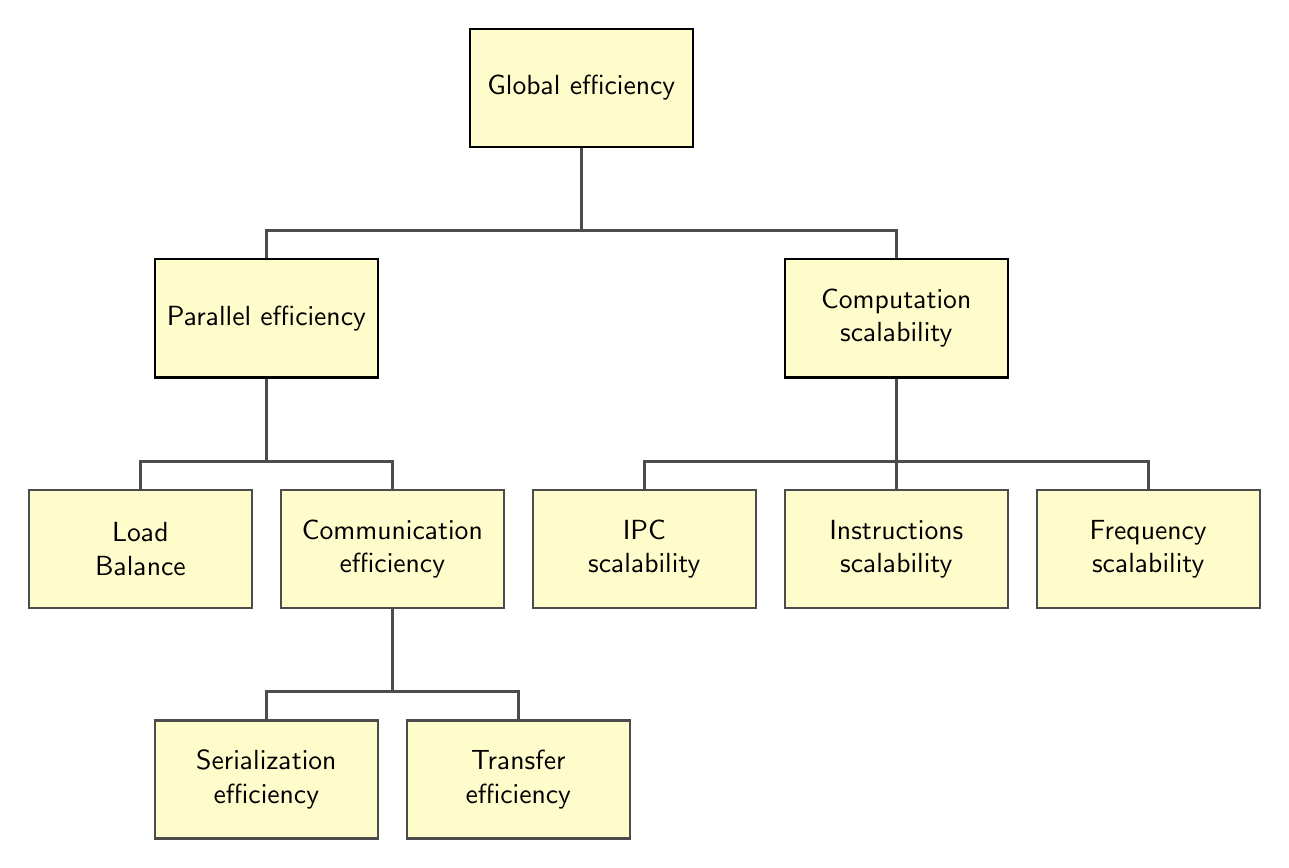
\begin{tikzpicture}[
% Label style
    label distance=3mm,
    every label/.style={blue},
% Event style
    event/.style={rectangle,thick,draw,fill=yellow!20,text width=2.6cm, minimum height=1.5cm,
		text centered,font=\sffamily,anchor=north},
% Children and edges style
    edge from parent/.style={very thick,draw=black!70},
    edge from parent path={(\tikzparentnode.south) -- ++(0,-1.05cm)
			-| (\tikzchildnode.north)},
    level 1/.style={sibling distance=8cm,level distance=1.4cm,
			growth parent anchor=south,nodes=event},
    level 2/.style={sibling distance=3.2cm},
    level 3/.style={sibling distance=3.2cm},
    level 4/.style={sibling distance=1cm}
%%  For compatability with PGF CVS add the absolute option:
%   absolute
    ]

  \node (glob) [event] {Global efficiency}
    child{node (par) {Parallel efficiency}
      child {node (lb) {Load  \\ Balance}}
      child {node (comm) {Communication efficiency}
        child {node (ser) {Serialization efficiency}}
        child {node (trans) {Transfer efficiency}}
      }
    }
    child{node (comp) {Computation scalability}
      child{node (ipc) {IPC \\ scalability}}
      child{node (ins) {Instructions scalability}}
      child{node (fre) {Frequency scalability}}
    };
\end{tikzpicture}
\caption{POP Efficiency metrics}
\label{popmet}
\end{figure}

The global efficiency describes how good is the parallelization in general. Then, the global efficiency is represented by:

\begin{itemize}
  \item \textbf{Parallel efficiency:} Shows the efficiency lost due to splitting the work between processes and the effects of adding communications.
  \item \textbf{Computation scalability:} Represents the efficiency lost due to computation side effects of the parallelization of the job. For example, dividing the data among processes adds more instructions, running with more processes in the same machine can lower the IPC because of the resource sharing.
\end{itemize}

\subsubsection{Parallel efficiency}

Before entering in-depth on the metrics, we need to explain a few assumptions. 
The efficiency metrics estimate that each process can be in two states:
\begin{itemize}
  \item Useful state means that the process is performing computation. We usually represent a process in useful with the colour blue.
  \item Not useful state means that the process does not perform computation, such as sending an MPI message or waiting in a synchronization. We usually represent a process that is not useful with the colour red.
\end{itemize}

Figure \ref{fig:usefulnot} shows the graphical representation in a timeline of processes and their states. The x-axis represents the time, y-axis processes, and the colour of a process means the state that the process is in that time. The Figure shows four processes following the pattern: All computing, processes 3, 2 and 1 finish early and wait for process 0, then process 0 finishes and re-establish the computation.

    \begin{figure}[htbp]
      \centering
      \begin{tracedraw}{0.6}
        \tracedrawAddToLegend(\large{Not-useful}, red)
        \tracedrawAddToLegend(\large{Useful}, blue)
        \tracedrawEnableLineName(\large{Process})
        \tracedrawSetLegendColorScale(0.5)

        \tracedrawSetLineHeight(0.7)
        \tracedrawAddChunk[color=gray, fill=blue](94)
        \tracedrawAddChunk[color=gray, fill=red](3)
        \tracedrawAddChunk[color=gray, fill=blue](3)

        \tracedrawNewLine

        \tracedrawAddChunk[color=gray, fill=blue](50)
        \tracedrawAddChunk[color=gray, fill=red](47)
        \tracedrawAddChunk[color=gray, fill=blue](3)

        \tracedrawNewLine
        
        \tracedrawAddChunk[color=gray, fill=blue](45)
        \tracedrawAddChunk[color=gray, fill=red](52)
        \tracedrawAddChunk[color=gray, fill=blue](3)

        \tracedrawNewLine
        
        \tracedrawAddChunk[color=gray, fill=blue](30)
        \tracedrawAddChunk[color=gray, fill=red](67)
        \tracedrawAddChunk[color=gray, fill=blue](3)

      \end{tracedraw}
      \caption[Example of useful and not useful states.]{Example of useful and not useful states. Own compilation}
      \label{fig:usefulnot}
    \end{figure}

    We define $E$ as the total execution time, $P = \{p_1,p_2,\dots, p_n\}$ as the set of processes and for each process the set of time intervals where the process is in useful $U_p = \{u_1^{p},u_2^{p},\dots,u_{|U|}^{p}\}$ and the same set but when the process is in not-useful $\overline{U}_p$. Equation \ref{eq:timeuseful} shows the definition of $T_{U_p}$ which is the total time the process is in useful. Graphically expressed the sum of the blue chunks. The time the process is in not-useful $T_{\overline{U}_p}$ is defined similarly.

    \begin{equation}\label{eq:timeuseful}
      T_{U_p}=\sum_{U_p}\textcolor{blue}{\blacksquare}=\sum_{i=1}^{|U_p|}u^p_{i} 
    \end{equation}

    The parallel efficiency ($PE$) represents the time lost due to the parallelization. Then we can express it as the factor of the total time in useful by the total CPU time consumed. As we said, as the metrics are multiplicative it can also be computed with the product of the Load Balance ($LB$) and the Communication Efficiency ($CE$). Equation \ref{eq:PE} shows the formalization.

    \begin{equation}\label{eq:PE}
      PE=\frac{\sum_{i=1}^{|P|} T_{U_i}}{E\ast|P|}=LB\ast CE
    \end{equation}

    The Load Balance measures the efficiency lost due to improper work distribution. Expressed mathematically the factor between the average time in useful by the maximum time in useful. Equation \ref{eq:LB} shows the formalization.

    \begin{equation}\label{eq:LB}
      LB=\frac{\sum_{i=1}^{|P|}T_{U_{i}}}{|P|\ast max^{|P|}_{i=1}T_{U_i}}
    \end{equation}
\subsubsection{Computation scalability}


